\begin{problem}[习题3.2]
用长分别为100, 200, 300, 400, 500, 600, 700, 800, 900, 1000的10个数组的排列来统计这两种算法的时间复杂性;
\end{problem}
\begin{solution}
\textbf{解:}测试程序见附录A,在linux下经g++编译运行得到如下结果:

\begin{figure}[!htb]
\centering
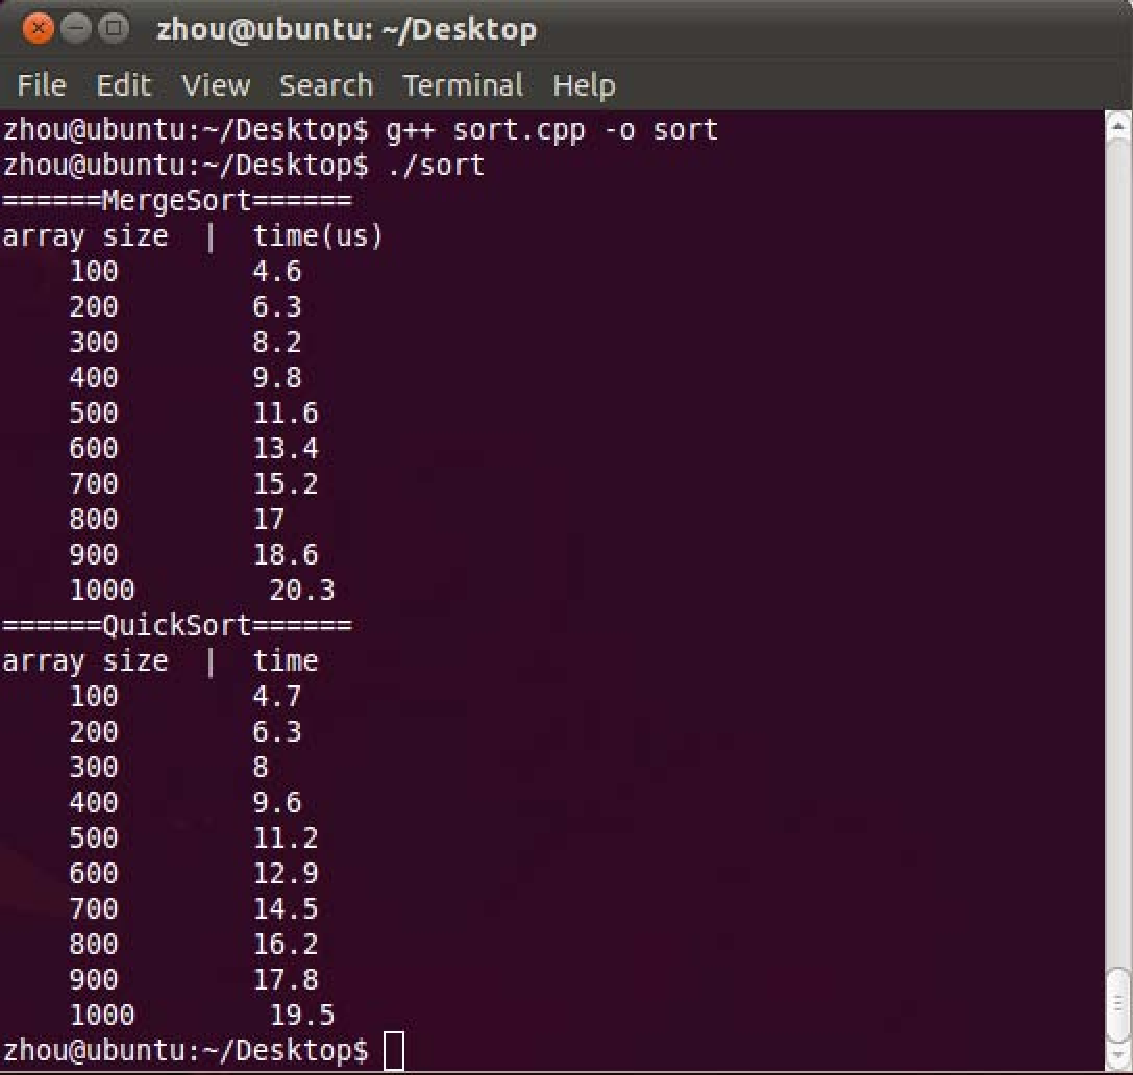
\includegraphics[width=0.5\textwidth]{result.pdf}
\caption{统计得到的两种算法的时间复杂性}
\end{figure}
\end{solution}
